
\noindent Вариант 2\\
1. $x=h-gh^2/(2v^2_0)=15,1$ м.\\
2. $a=g(m_2-m_1)/(m_1+m_2)=5$ м/с$^2$\\
3. $F=A/(s\ cos\ \alpha)=50$ Н.\\
4. $l=m^2v^2/(2\mu gM^2)=2$ м.\\
5. $V=vRT/p=9.3$ м$^3$,\ \ \ \ \ \ где $R=8,31$ Дж/\\ /(моль$\cdot$ К) $-$ универсальная газовая постоян-\\ ная.\\
6. $\tau=m(c\Delta t +\lambda)/P=5474$ с.\\
7. $q=S\varepsilon R/(R+r)=10$ мкФ.\\
8. $F=q^2/(4\pi \varepsilon_0 r^2)=9\cdot10^3$ Н.\\
9. $m_1/m_2=(r_1/r_2)^2=4$.\\
10. $\alpha=30^\circ$.\\ \\

\noindent Калейдоскоп <<Кванта>>\\
(ФК <<Квант>> № 2)\\

\noindent Вопросы и задачи\\
1. Свет, испускаемый лазером,$-$почти строго\\ параллельные лучи.\\
2. Для разных длин световых волн по-\\ казатели преломления вещества различны.\\
3. Ближе у перпендикуляру$-$красный луч,\\ дальше всех$-$фиолетовый.\\
4. Для любой линзы главное фокусное\\ расстояние больше (по модулю) для красных\\ лучей.\\
5. Зеленое.\\
6. Красный, поскольку при переходе из одной\\ среды в другую частота света, определяю- \\ щая цвет лучей, не изменяется.\\
7. Нет, поскольку сама интерференция —\\ следствие принципа суперпозиции, согласно ко- \\ торому фронты волн, «проникающих» одна в\\ другую, взаимно не деформируются.\\
8. Да, так как прямая и обратная волны\\ когерентны.\\
9. Из-за стенания воды нижняя часть плен-\\ ки утолщается, а верхняя становится тоньше.\\ Поэтому соответствующие интерференционные\\ полосы смещаются.\\
10. Из за дифракции на краях Луны на поверх-\\ ности Земли появляется интерференционная\\ картина.\\
11, 12. Начинают сказываться дифракцио -\\ ные явления.\\

\noindent Микроопыт\\
В щель будут видны темные дифракционные\\ полосы: четкая полоса в центре и ряд более\\ слабых боковых.\\ \\ \\ 

\noindent Квант для младших школьников\\
(МК <<Квант>> №2)\\ 

\noindent 1. На весах 300 монет.\\ \\ 
2. См. рис. 3. Сумма $S$ чисел на каждой окруж-\\ности равна 12, так как $4S=36+S$.\\
3. См. рис. 4.\\
4. Ошибка в графе <<Разность мячей>> у коман-\\ ды Швеции: при одном выигрыше и одной\\
ничьей разность мячей не может быть <<$1-1$>>.\\ Общее количество забитых мячей рано 11,\\


\begin{table}[t]
\begin{tabular}{ll}
    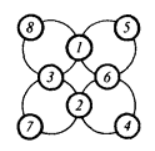
\includegraphics[scale=0.4]{image1.png} & 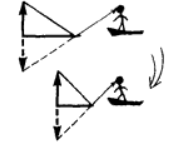
\includegraphics[scale=0.4]{image2.png}\\
\end{tabular}
\end{table}
\noindent\textit{Рис. 3.\ \ \ \ \ \ \ \ \ \ \ \ \ \ \ \ \ \ \ \ \ \ \ \ \ \ \ Рис. 4.}\\

\noindent а число пропущенных - 12. Поэтому ошибка\\
в счете на 1 мяч, т. е. разность мячей\\
Швеции равна <<2 - 1>>, либо <<1 - 0>>. Рассмот-\\
рение этих вариантов приводит к следующей\\
таблице:


\begin{table}[h]
{\footnotesize
\begin{tabular}{|p{1.2cm}|p{0.7cm}|p{0.7cm}|p{0.45cm}|p{0.45cm}|p{0.8cm}|p{0.55cm}|p{0.35cm}|}
    \hline
        & Венгр. & Швец. & Исп. & Ирл. & Франц. & Разн. мяч. & Оч-ки\\
    \hline
    &&&&&&&\\ 
    Венгрия &\ \ \ *    &\ \ \ $-$ &\ \ $-$ &\ 2:1   &\ \ 2:0     & 4 - 1 &\ 4\\
    Швеция  &\ \ \ $-$   &\ \ \ *   &\ 1:1   &\ 1:0   &\ \ \ $-$   & 2 - 1 &\ 3\\
    Испания &\ \ \ $-$ &\ \ 1:1   &\ \  *  &\ 2:2   &\ \ \ $-$   & 3 - 3 &\ 2\\
    Ирландия &\ \ 1:2   &\ \ 0:1   &\ 2:2   &\ \ *   &\ \ \ $-$   & 3 - 5 &\ 1\\
    Франция &\ \  0:2   &\ \ \ $-$ &\ \ $-$ &\ \ $-$ &\ \ \ *     & 0 - 2 &\ 0\\ 
    &&&&&&&\\
    \hline
\end{tabular}
}
\end{table}


\noindent 5. Разрежем четырехугольник по средним ли-\\
ниям и сложим полученные четырехугольники\\
так, чтобы вершины большого четырехуголь-\\ \\ \\ \\ \\ \\ \\ \\

\noindent\textbf{{\LARGE АНКЕТА 3$-$89}\\ \\
Дорогой читатель!}\\
Ежегодно в последнем номере журнала мы\\
помещали <<Нашу анкету>>. Но нам пришло\\
в голову, что легче, проще высказать свое\\
мнение, что называется, по свежим следам.\\
Поэтому мы решили помещать анкету раз в\\
квартал.\\
Мы обращаемся к Вам с просьбой. Ответьте,\\
пожалуйста, на вопросы анкеты (на те, на\\
которые Вы хотите и можете ответить), вы-\\
режьте анкету и пришлите в редакцию; на\\
конверте напишите <<АНКЕТА 3$-$89>>.\\
Очень надеемся на обратную связь.\\ \\
1. Класс, в котором Вы учтесь: \underline{\hspace{3cm}}\\
Ваша профессия (если Вы работаете): \underline{\hspace{2cm}}\\
\underline{\hspace{7.86cm}}\\
круг Ваших интересов: физика, матема-\\
тика, астрономия, космонавтика, инфор-\\
матика (подчеркните).\\
2. Какие разделы журнала для Вас наиболее\\
интересны? \underline{\hspace{6cm}}\\
\underline{\hspace{7.86cm}}\\

\begin{flushright}
\textit{(см. с. 80)\ \ \ \ \ \ \ }
\end{flushright}
